\subsection{Descripci\'on del problema}

En este punto se nos pide resolver el problema de ubicar centrales de gas de manera estrat\'egica entre los pueblos de una cierta regi\'on.\\

Dados $n$ pueblos con sus respectivas coordenadas en el plano y $k$ centrales de gas, la idea es decidir en qu\'e pueblos ubicar las centrales. Adem\'as es posible construir tuber\'ias entre pueblos: una tuber\'ia que va de un pueblo con central a uno sin no s\'olo transporta el gas a este \'ultimo sino que adem\'as lo convierte en potencial proveedor. Es decir que se da una especie de transitividad entre los pueblos: si un pueblo $a$ con central de gas se conecta a otro pueblo $b$ y a su vez $b$ se conecta con $c$ entonces $c$ tambi\'en recibe gas (y puede distribuirlo).\\

El \'unico problema que presentan las tuber\'ias es que, a mayor longitud aumenta la posibilidad de rotura de las mismas. Evidentemente \'este es un factor que se quiere evitar, por lo cual se nos pide que, al elegir los pueblos donde instalar las centrales y y las conecciones entre los mismos minimicemos el tama\~no de la tuber\'ia m\'as larga.\\

Veamos algunos ejemplos, la siguiente es una situacion trivial en la que tenemos la misma cantidad de pueblos que de centrales:

\begin{figure}[h]
\begin{center}
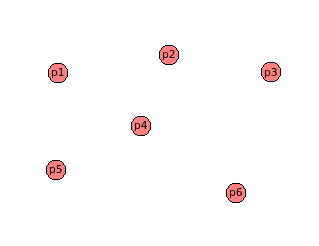
\includegraphics[scale=0.7]{./img/ej2_explicacion1.png}
\caption{Caso trivial}
\end{center}
\end{figure}

Los circulos colorados indican donde fueron instaladas las centrales, en este caso no hay ninguna tuber\'ia.\\

Veamos el siguiente caso mas complejo: 

\begin{figure}[h]
\begin{center}
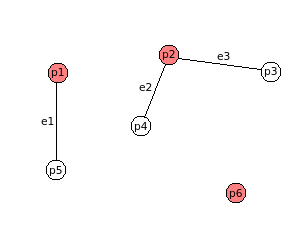
\includegraphics[scale=0.7]{./img/ej2_explicacion2.png}
\caption{Caso con K = 3 y N = 6}
\end{center}
\end{figure}

Como dato, sabemos que $e_2 < e_3 < e_1$ con lo cual nuestro largo m\'aximo de tuber\'ia es $e_1$

\subsection{Resoluci\'on}

Para la resoluci\'on del problema decidimos primero modelarlo con grafos, de forma que los nodos representen los pueblos, y las aristas (con pesos) las posibles conexiones entre pueblos. Los pesos est\'an dados por las distancias entre cada par de pueblos. \\

Como se nos pide minimizar el riesgo de rotura de las tuber\'ias a instalar, lo ideal ser\'ia lograr un esquema de conexiones tal que el largo de la tuber\'ia mas larga sea m\'inimo. Como veremos m\'as adelante, la ubicaci\'on de las centrales de gas no es de gran importancia ya que la transimisi\'on del servicio de gas se da por transitividad entre pueblos conectados (mientras alguno de ellos tenga una central). Por lo tanto lo importante es tener grupos de pueblos conectados a una misma central de manera que las tuber\'as necesarias sean de tama\~no m\'inimo. \\

Para obtener el esquema de conexiones antes mencionado partimos de pensar la regi\'on como un grafo completo; es decir que suponemos que todas las ciudades est\'an conectadas entre s\'i. Luego, a partir del grafo completo la idea es obtener un \'arbol generador m\'inimo del mismo utilizando el algoritmo de Prim.\\
Finalmente cortamos las $k - 1$ aristas m\'as largas del \'arbol, obteniendo un grafo de $k$ componentes conexas tal que la arista m\'as larga del grafo es de peso m\'inimo.\\ 
Como se dijo antes, es indistinto cu\'al de los pueblos de cada componente conexa tiene instalada la central. Sin embargo, como el ejercicio pide especificar el pueblo elegido, instalamos inicialmente una central en la ra\'iz del \'arbol. Luego, por cada arista ($v_1$, $v_2$) que eliminamos instalamos una central en el pueblo representado por $v_2$. %TODO: aclarar por que anda

\subsubsection{Implementaci\'on de Prim}
Describimos a continuaci\'on nuestra implementaci\'on del algoritmo de Prim.\\

Elegimos como ra\'iz del \'arbol generador m\'inimo al primer pueblo de la lista de pueblos de la regi\'on. Como al menos va a haber una central, instalamos una en el pueblo ra\'iz.\\
Luego realizamos un ciclo que se repite $n - 1$ veces (siendo $n$ la cantidad de nodos, es decir, ciudades), en el cual en cada iteraci\'on obtenemos el nodo m\'as cercano al \'arbol y lo agregamos al mismo.\\
Para saber cu\'al es el nodo m\'as cercano al \'arbol debemos, en cada iteraci\'on calcular la distancia m\'inima entre cada nodo que no pertenece al \'arbol y los que s\'i pertenecen.\\
Como partimos de un \'arbol que s\'olo tiene al primer nodo de la lista ($n_0$) inicialmente calculamos la distancia de cada uno de los nodos restantes a $n_0$. Luego se elegimos el nodo de menor distancia y lo agregamos al \'arbol y repetimos el proceso de calcular distancias y elegir el nodo m\'as cercano.\\
As\'i ,cada vez que agregamos un nodo al \'arbol volvemos a computar la m\'inima distancia de los nodos restantes comparando la distancia que cada uno tiene guardada como m\'inima con la distancia al nuevo nodo.\\
Una vez agregados todos los nodos al \'arbol tenemos un \'arbol generador m\'inimo.\\

\newpage

\subsection{Demostraci\'on de la resoluci\'on}

Veamos que: sea T un \'arbol generador m\'inimo, eliminar las k-1 aristas de mayor peso nos da un bosque de k componentes de riesgo m\'inimo.\\

\subsubsection{Caso base - k = 1}

Queremos ver que para el caso de k=1, dado el grafo de n ciudades, cualquier AGM de ese grafo es un \'arbol generador de riesgo m\'inimo.\\
En este caso, como k=1, k-1=0 no hay que eliminar ninguna arista; basta con ver que el AGM es de riesgo m\'inimo.\\

Llamemos $T$ al AGM y supongamos que existe otro \'arbol generador $T'$ que tiene un riesgo menor que $T$. Sea $e = (n_i, n_j)$ la arista de peso m\'aximo de $T$ ($peso(e) == riesgo(T)$ \footnote{$riesgo(T) = \max_{e \in T} peso(e)$}), queda claro que \footnote{$riesgo(T') < riesgo(T) \Rightarrow \max_{e \in T'} peso(e) < \max_{e \in T} peso(e) \Rightarrow (\forall e' \in T')\, peso(e') < peso(e)$}:
\begin{equation}\label{eq}
(\forall e' \in T')\, peso(e') < peso(e)
\end{equation}
Entonces, me puedo armar un \'arbol $T''$ tal que $peso(T'') < peso(T)$ de la siguiente manera:

\begin{itemize}
 \item Elimino de $T$ la arista $e = (n_i, n_j)$. Luego, el \'arbol generador se parte en exactamente dos componentes conexas, la que posee al nodo $n_i$ y la que posee al nodo $n_j$.
 \item Sabemos que existe una arista $e'$ en $T'$ que une ambas componentes conexas, ya que $T'$ es un AG del mismo grafo del que $T$ es un AGM (con lo cual $V(T) == V(T')$ y adem\'as $T'$ es conexo por ser un AG). Por \'ultimo, notemos que $e' \neq e$ pues $peso(e') < peso(e)$ por (\ref{eq}). Entonces puedo unir ambas componentes con $e'$ y esto no me genera ciclos (ya que estoy uniendo dos componentes conexas distintas).
\end{itemize}
Notar que si hay m\'as de una arista $e$ debemos eliminarlas tambi\'en y hacer el intercambio por su correspondiente en $T'$. 
Con esto, obtenemos un \'arbol generador $T''$ tal que $peso(T'') < peso(T)$, pero esto es \textbf{absurdo} ya que estabamos suponiendo que $T$ era un AGM. El absurdo proviene de suponer que existe un AG con riesgo m\'inimo que no es AGM.\\

\subsubsection{Paso inductivo}

Suponemos ahora que vale P(k) = eliminar las k-1 aristas de mayor peso nos da un bosque de k componentes de riesgo m\'inimo, $(\forall k \leq n)$. Queremos ver que vale P(k+1).\\

\begin{itemize}
\item Caso $k + 1 \geq n$. En este caso vamos a cortar todas las aristas del \'arbol, terminando con n componentes de grado 0, es decir riesgo = 0. Es trivial ver que el riesgo en este caso es m\'inimo y que ningun otro AG lo podr\'ia mejorar.
\item Caso $k + 1 < n$. Por HI sabemos que los \'arboles formados por las k primeras eliminaciones de aristas (siempre de mayor a menor) son de riesgo m\'inimo.\\
Podemos entonces, de todos los \'arboles formados, concentrarnos en el que tiene la arista de mayor peso; que es la que se elimina en el paso k + 1. Llamemoslo $B$\\
En el caso base probamos que $T$ el \'arbol generador m\'inimo sobre el cual estamos trabajando es de riesgo m\'inimo. En particular sabemos que no hay ninguna arista de $B$ que pueda ser reemplazada por otra de menor peso.\\
Adem\'as, por HI sabemos que $B$ es de riesgo m\'inimo, ya que se obtuvo de eliminar k aristas de $T$.\\
Ahora, si eliminamos $e = (n_i, n_j)$ la arista de peso m\'aximo de $B$, obtenemos dos \'arboles, de los cuales al menos uno tiene a $e' = (n_i', n_j')$, la arista de $B$ que le sigue inmediatamente en peso a $e$ (es decir que $peso(e') \leq peso(e) = (n_i, n_j)$).\\
Es decir que pasamos de $B$ un \'arbol de riesgo $peso(e)$ a $B', B''$ dos \'arboles cuyo riesgo es, a lo sumo $peso(e)$; y el riesgo sigue siendo m\'inimo ya que es menor o igual al que ten\'iamos antes.\\ 
\end{itemize}

\subsection{Complejidad del algoritmo}

Veamos la complejidad del algoritmo propuesto utilizando un pseudoc\'odigo que facilite el an\'alisis.

\begin{itemize}
\item poner puebloNuevo $\leftarrow$ primer pueblo de la lista
\item agregar a arbolPueblos $\leftarrow$ (puebloNuevo, puebloNuevo)
\item instalar central en puebloNuevo y poner centralesInstaladas $\leftarrow$ 1
\item poner i $\leftarrow$ 0
\item mientras i < cantidadPueblos - 1 (Agregamos los pueblos uno a uno, n iteraciones)
\begin{itemize}
	\item actualizarDistancias respecto a puebloNuevo (Lo analizamos m\'as adelante, toma O(n))
	\item poner masCercano $\leftarrow$ pueblo mas cercano fuera del arbol
	\item poner cercanoEnArbol $\leftarrow$ pueblo del arbol con el que masCercano tiene distancia minima
	\item agregar arbolPueblos $\leftarrow$ (cercanoEnArbol, masCercano) (Agregar un elemento a una lista es O(1))
\end{itemize}
\item ordenar arbolPueblos de mayor a menor por distancia entre pares 
\item mientras centralesInstaladas < cantidadCentralitas (k iteraciones, que a lo sumo son n)
\begin{itemize}
	\item poner aristaMayor $\leftarrow$ primer elem de arbolPueblos
	\item instalarCentral(aristaMayor.segundo)
	\item eliminar aristaMayor de arbolPueblos (eliminar usando erase es O(1))
\end{itemize}
\end{itemize}

Como se puede ver, la complejidad est\'a dada por el primer ciclo, el cual hace n iteraciones (donde n corresponde a la cantidad de ciudades), ya que debe agregarlas una a una al \'arbol generador m\'inimo. Dentro de ese ciclo se actualizan las distancias de las ciudades al \'arbol; veremos la complejidad de hacerlo a continuaci\'on, pero podemos adelantar que realiza n iteraciones tambi\'en. Con lo cual la complejidad total del ciclo quedar\'ia en O(n).\\
Una vez obtenido el \'arbol lo ordenamos de mayor a menor, donde el par ($v_1$, $v_2$) es mayor a otro ($w_1$, $w_2$) si la distancia entre $v_1$ y $v_2$ es mayor a la distancia entre $w_1$ y $w_2$. Ordenar una lista con std::list::sort toma O(n*log(n)). \cite{sort}\\
Finalmente eliminamos los primeros k-1 (donde k es el n\'umero de centrales) pares de pueblos; es decir los pares que tienen mayor distancia. Cada eliminaci\'on toma O(1) usando std::list::erase \cite{erase}. En total toma O(k), que es a lo sumo O(n).\\

Vemos ahora el pseudoc\'odigo de actualizarDsitancias para confirmar que es O(n).\\

\begin{itemize}
\item poner puebloNuevo.distanciaAlArbol $\leftarrow$ 0
\item para cada pueblo en pueblos (iteramos todos los pueblos, O(n))
\begin{itemize}
	\item poner distanciaActual $\leftarrow$ pueblo.distanciaAlArbol
	\item si distanciaActual es mayor a 0 (el pueblo no es parte del arbol)
	\begin{itemize}
		\item poner distanciaNueva $\leftarrow$ distancia(puebloNuevo, pueblo)
		\item si distanciaNueva > distanciaActual poner pueblo.distanciaAlArbol $\leftarrow$ distanciaNueva
	\end{itemize}
\end{itemize}
\end{itemize}

En actualizarDistancias es claro que la complejidad est\'a dada por la iteraci\'on a trav\'es de las ciudades, es decir O(n). Luego, dentro del ciclo s\'olo se realizan comparaciones y asignaciones, que no afectan la complejidad significativamente.\\

Podemos decir ahora que la complejidad del algoritmo est\'a dada por el ciclo en el que se agregan nodos al \'arbol y que la misma es O($n^2$).

\newpage

\subsection{C\'odigo fuente}

\lstset{language=C++,
                basicstyle=\ttfamily\footnotesize,
                keywordstyle=\color{blue}\ttfamily,
                stringstyle=\color{red}\ttfamily,
                commentstyle=\color{green}\ttfamily,
                morecomment=[l][\color{magenta}]{\#},
                breaklines=true
}
\begin{lstlisting}

/* Constructor de region */
Region::Region(list<Pueblo*> * lista_pueblos, int centralitas){
	
	_centralitas = centralitas;
	_centrales_instaladas = 0;
	_tuberias_instaladas = 0;
	_pueblos = lista_pueblos;
	_arbol_pueblos = new list<pair<Pueblo*, Pueblo*> >();

}

void Region::resolver(){

	int cantPueblos = _pueblos->size();
	
	// Uso Prim para agregar pueblos al arbol

	// Elijo la primera ciudad de la lista como root
	Pueblo* puebloNuevo = *_pueblos->begin();
	pair<Pueblo*, Pueblo*> parPueblos = pair<Pueblo*, Pueblo*>(puebloNuevo, puebloNuevo);
	_arbol_pueblos->push_back(parPueblos);
	// Inicialmente solo el pueblo root tiene una central instalada
	puebloNuevo->instalarCentral();
	_centrales_instaladas = 1;

	// Pueblo mas cercano actual
	Pueblo * masCercano = puebloNuevo;

	// Agrego ciudades al arbol de a una - O(n)
	for(int i=0; i<cantPueblos-1 ; i++){
		
		// Actualizo las distancias al arbol y me quedo con la menor
		//cout << "nuevo_id: " << puebloNuevo->getId() << endl;
		masCercano = actualizarDistancias(puebloNuevo);

		// Agrego masCercano al arbol
		// En la proxima iteracion la distancia va a quedar en 0
		parPueblos = pair<Pueblo*, Pueblo*>(masCercano->getPuebloCercano(), masCercano);
		_arbol_pueblos->push_back(parPueblos);
		puebloNuevo = masCercano;
	}

	// Ordeno los pares de ciudades segun distancia (de mayor a menor)
	_arbol_pueblos->sort(compararDistancia);

	// Mientras que pueda instalar centrales achico el tam maximo de las tuberias
	// Es decir, genero k componentes conexas, cada una con una central

	list<pair<Pueblo*,Pueblo*> >::iterator p = _arbol_pueblos->begin();
	while (p != _arbol_pueblos->end()){
		if(_centrales_instaladas<_centralitas){
			// p representa la tuberia mas larga, la elimino e instalo una nueva central
			if(!((*p).second)->tieneCentral()){
				((*p).second)->instalarCentral();
				_centrales_instaladas+=1;
			}
			p = _arbol_pueblos->erase(p);
			
		}else{
			p++;
		}
	}
}

// Actualiza distancia minima al arbol de cada pueblo y devuelve el mas cercano
Pueblo* Region::actualizarDistancias(Pueblo* puebloNuevo){

	double distActual;
	double distNueva;
	double min = std::numeric_limits<double>::infinity();
	Pueblo* masCercano = puebloNuevo;

	// Antes de empezar actualizo la distancia del nuevo pueblo
	puebloNuevo->setDistanciaArbol(0.0);

	// Recorro todos los pueblos y actualizo sus distancias al arbol comparando con el ultimo p agregado
	for(list<Pueblo*>::iterator p = _pueblos->begin(); p != _pueblos->end(); p++){

		distActual = (**p).getDistanciaArbol();

		// Si no pertenece al arbol actualizo
		if(distActual > 0.0){

			distNueva = (**p).distancia(*puebloNuevo);
			
			if(distNueva < distActual){
				(**p).setPuebloCercano(puebloNuevo);
				(**p).setDistanciaArbol(distNueva);
			}

			distActual = (**p).getDistanciaArbol();

			// Si es el menor hasta el momento guardo la ciudad
			if(distActual < min){
				masCercano = *p;
			}
		}
	
	}

	return masCercano;
}

\end{lstlisting}

\subsection{Casos de prueba}

Como casos de prueba para el algoritmo elegimos inputs de los siguientes tipos:
\begin{itemize}
\item Caso en los que la cantidad de pueblos es igual a la cantidad de centrales.
\item Caso en los que la cantidad de pueblos es menor a la cantidad de centrales.
\item Caso en el que cada ciudad est\'a a distancia 1 de la siguiente.
\end{itemize}

Los casos utilizados se encuentran en el directorio /ej2/inputs/prueba y se puede verificar que funcionan ejectuando, desde /ej2, ./ej2 > inputs/prueba/algunCaso.txt.

\subsection{Performance}

Para el an\'alisis de performance de este ejercicio decidimos ejecutar lotes aleatorios de tests siguiendo los siguientes criterios:

\begin{itemize}
	\item Iteramos entre 50.000 y alrededor de 80.000 pueblos.
	\item En cada iteraci\'on incrementamos la cantidad de pueblos en 1.000 unidades.
	\item Generamos un input con coordenadas aleatorias de los pueblos.
	\item Para cada iteraci\'on tomamos los siguientes valores de centrales:
	\begin{itemize}
		\item Comenzamos desde 1 central hasta 100.000.
		\item Incrementamos en cada iteraci\'on la cantidad de centrales en 4.000 unidades
	\end{itemize}
\end{itemize}

Para realizar esto generamos dos scripts de bash, uno que va iterando la cantidad de pueblos y centrales y por cada caso invoca al otro script, quien se encarga de generar las coordenadas aleatorias para la cantidad de pueblos deseada.

En cuanto a las cantidades de pueblos y centrales entendimos que para evitar la aleatoriedad en los resultados deb\'iamos ejecutar una gran cantidad de casos e ir incrementando la cantidad de pueblos hasta un n\'umero considerable. 
Adem\'as, nos pareci\'o interesante pasar por distintas cantidades de centrales, empezando por una, en la cual no iban a ser necesarios recortes de conexiones entre pueblos, e ir incrementando los valores hasta llegar a cantidades similares a la de pueblos, en donde iba a ser conveniente realizar m\'as recortes por ende la implementaci\'on iba a tener que realizar m\'as procesamiento y poder visualizar as\'i que la complejidad no se ve\'ia afectada.

\begin{center}
\begin{figure}[h!]
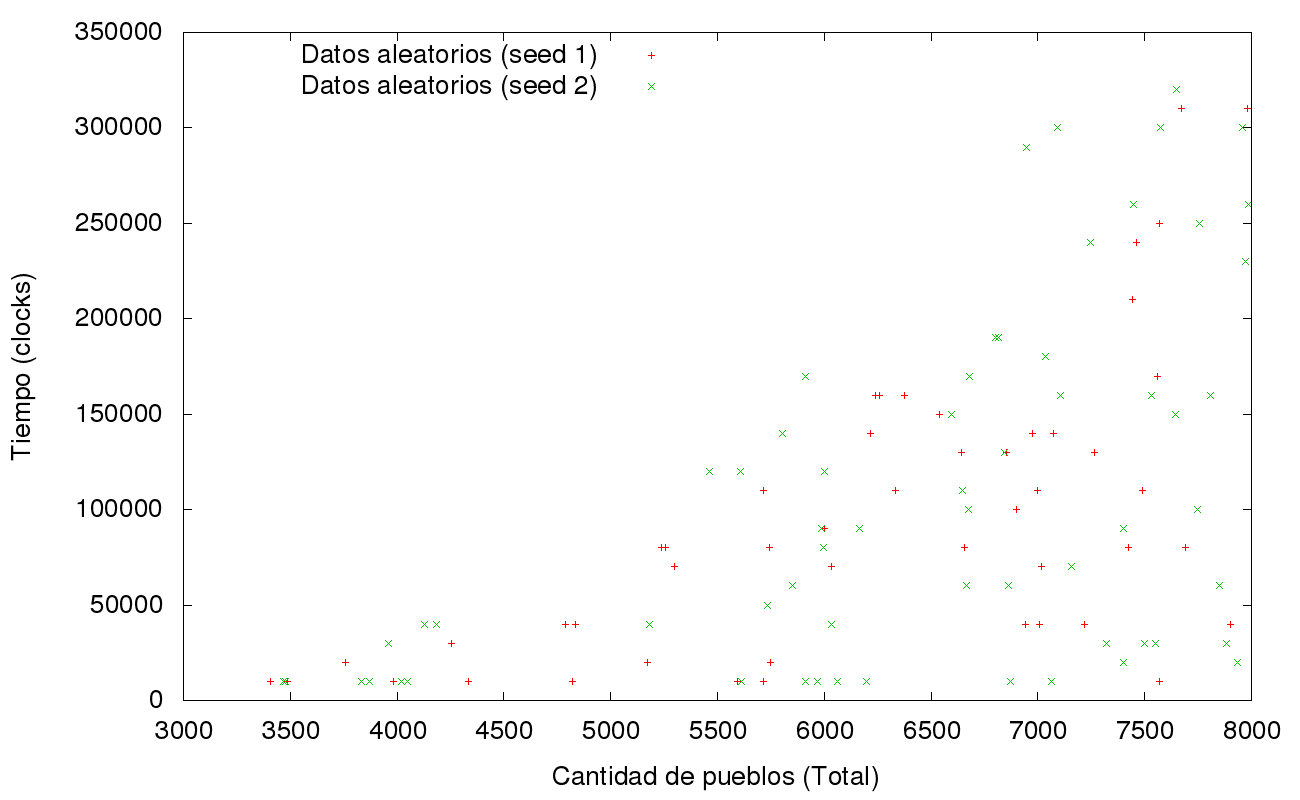
\includegraphics[scale=0.4]{./img/ej2_chart.png}
\caption{Tiempo transcurrido por cantidad de pueblos}
\end{figure}
\end{center}





Como podemos observar, con los datos obtenidos de las ejecuciones, se genera un gr\'afico con, a priori, la pinta de una funci\'on cuadr\'atica. 

Para poder observar este comportamiento mejor es necesario acompanarlo por la funci\'on $c*n*n$ con $c$ constante tal que permita ajustar la funci\'on cuadr\'atica al gr\'afico generado.

Para poder obtener dicha constante multiplicamos cada $n$, cantidad de pueblos, por si mismo y luego dividimos el tiempo resultante por dicho valor. De esta manera obtenemos una relaci\'on entre el cuadrado de la cantidad de pueblos y el tiempo de ejecuci\'on para cada valor. 
Finalmente, tomando un valor de $c$ apenas m\'as grande que el mayor obtenido en las anteriores operaciones, podemos aproximarnos a una constante que nos permita visualizar con mayor claridad que la complejidad solicitada no es superada y que el comportamiento se asemeja al deseado/solicitado.

Como peque\~na aclaraci\'on vale decir que los saltos que se producen en el eje x en el gr\'afico se corresponden con que ibamos iterando la cantidad de pueblos de mil en mil y es por eso que no se observan valores intermedios. 
As\'i tambi\'en, podemos observar que los distintos valores de tiempo para una misma cantidad de pueblos se corresponden con resultados para distintas cantidades de centrales.

Siguiendo por esta l\'inea de an\'alisis, entre los 55.000 y los 65.000 pueblos se puede notar una gran densidad en los valores, indicandonos que para dichas cantidades de pueblos, los tiempos de ejecuci\'on no se ven afectados por la cantidad de centrales.
